
% Dies ist der "Zentral-Dokument", die verschiedenen Teile k�nnen Sie
% unten einf�gen (s.u.). 
%
 
%[Schritgr��e, Seitenlayout, Papierformat, Satzspiegel, Bindungs-Korrektur-Ma�]
\documentclass[12pt, twoside, a4paper, DIV12, BCOR16mm]{scrartcl}

%L�ndereinstellungen
\usepackage[german,english]{babel}

%Grafiken, erweiterte Kopf- und Fu�zeilen, Seienreferenzvariablen, Listings, erweiterte Symbole,
%deutsche Literatur Formatierung, zeilen-�bergreifende Kommentare, Textmarkierungen
\usepackage{graphicx, fancyhdr, lastpage, listings, wasysym, 
            bibgerm, comment, changebar} 

% weiter evtl. n�tzliche Packages: ifthen, wasysym, changebar, supertabular

%\usepackage{palatino}% weitere Schriftarten

\usepackage[latin1]{inputenc} % Umlaute richtig verarbeiten  
\usepackage[T1]{fontenc}      % Feinheiten im Satz von Umlauten

% Packages, die 'bessere' PDF-Dokumente erzeugen 
\usepackage{ae} 
\usepackage[
        pdftitle={Beispiel Thesis}
        bookmarks=true,
        bookmarksnumbered=true, % Verwendete Bookmarks anzeigen
        colorlinks,   % Farbige Links
        linkcolor=black,
        urlcolor=blue,
        citecolor=black]{hyperref}
%\usepackage[dvips]{thumbpdf}

\pagestyle{fancy}

% Legt die Einr�cktiefe der ersten Zeile f�r aller Abs�tze fest. (0:=Abs�tze nicht einr�cken)
\setlength{\parindent}{0pt}  
%\parskip1ex plus0.5ex minus0.5ex   

% Legt die Breite des Randnotizen-Bereichs festlegen (auch �ber BCORxxx konfigurierbar)
%\setlength{\marginparwidth}{25mm}
%\evensidemargin0mm
%\oddsidemargin8mm

% Definiert die Gesamth�he des Textrumpfes f�r alle nachfolgenden Seiten.
\setlength{\textheight}{225mm}
\setlength{\headheight}{13mm}
\setlength{\topskip}{10mm}

% Nummerierungstiefe des Inhaltsverzeichnis 
\setcounter{tocdepth}{2} % auch {3} ist OK aber bitte nicht mehr

% Kopfzeilenformatierung
%\fancyhead[RO,LE]{\small \sffamily Inhalt} 
%\fancyhead[LO,RE]{\small \sffamily Beispiel f�r ein \LaTeX\ Dokument} 


%
% texAbbrev.tex: Einige Abk�rzugen 
%

\newcommand{\ia}{i.\,Allg.\ }
\newcommand{\dht}{d.\,h.\ }
\newcommand{\ua}{u.\,a.\ }
\newcommand{\so}{s.\,o.\ }
\newcommand{\zb}{z.\,B.\ }
\newcommand{\zbdp}{z.\,B.:\ }
\newcommand{\idr}{i.\,d.\,R.\ }
\newcommand{\zt}{z.\,T.\ } 
\newcommand{\zz}{z.\,Zt.\ } 
\newcommand{\igs}{i.\,Ggs.\ } 

\newcommand{\code}{\ttfamily}

\newcommand{\svs}{\vspace*{0.5ex}} 
\newcommand{\myrule}{\ \vspace{1ex} \\ \hrule} 
\newcommand{\figref}[1]{Abb.~\ref{#1}} 
\newcommand{\secref}[1]{Abschnitt~\ref{#1}} 
\newcommand{\mymargin}[1]{\marginpar{\raggedright \footnotesize \sffamily #1}} 

\renewcommand{\topfraction}{0.95}
\renewcommand{\bottomfraction}{0.95}

\newenvironment{trilist}{
    \renewcommand{\labelitemi}{\(\triangleright\)}
    \renewcommand{\labelitemii}{{\bfseries -}}
    \setlength{\partopsep}{0ex plus .5ex minus .5ex} 
    \setlength{\topsep}{-1ex plus .5ex minus .5ex} 
    \setlength{\parskip}{1.2ex plus .5ex minus .5ex}
    \setlength{\itemsep}{0pt plus .5ex minus .5ex}
    \setlength{\parsep}{0pt plus .5ex minus .5ex} 
    \begin{itemize}
    }
   {\end{itemize}}

 % eigene Kommandos laden 


\begin{document} 

\includecomment{comment}
\excludecomment{unsinn1} % ben�tigt das Package "comment". Ein- und Auschalten von Textteilen z.B. Anmerkungen 
\begin{unsinn1} 
Hier steht ein unsinniger Text, welcher aber gl�cklicher Weise nicht angezeigt wird!!!
\end{unsinn1} 

%Titelseite
\begin{titlepage}
\sffamily
\setlength{\tabcolsep}{0mm}
\begin{tabular*}{\textwidth}{l@{\extracolsep\fill}r} 

%\hspace{-0.4cm}
%
\includegraphics[width=6cm]{Bilder/logo_welle_en}  % Englische Version des Logos 

\includegraphics[width=5cm]{Bilder/rwu} % Deutsche Version des Logos

  &
\raisebox{3mm}{
	\begin{tabular}{r}
%\rule{0cm}{0.5cm}
Course Applied Computer Science\\[0.5mm]
School of Electrical engineering and Computer Science\\
\end{tabular}}
\end{tabular*}
\setlength{\tabcolsep}{6pt}

\vspace*{4cm}
\begin{center}
\textbf{\Large{Bachelor-Thesis}}\\
\vspace*{1cm}
\textbf{\LARGE{Self-supervised training of a neural network for obstacle avoidance}}\\
\vspace*{2cm}
\large{for the purpose of obtaining the degree}\\[2mm]
\large{Bachelor of Applied Computer Science}\\
\end{center}

%\vfill
\vspace{2cm}
\begin{center}

	submitted by:\\[5mm]
{\Large Martin Samuel Lanz} \\[5mm]
    \today \\[3cm]
{\normalsize
	\begin{tabular}{rl}
	1. Gutachter: 	& Prof. Dr. Markus Schneider\\
	2. Gutachter: 	& M.Sc. Benjamin St�hle 
	\end{tabular}
}
\end{center}

\end{titlepage}


%Eidesstattliche Erkl�rung
\begin{newpage}
\vspace*{\fill}
\section*{Eidesstattliche Erkl�rung}
Hiermit versichere ich, die vorliegende Arbeit selbststndig und unter ausschlielicher Verwendung der angegebenen Literatur und Hilfsmittel erstellt zu haben. Die Arbeit wurde bisher, in gleicher oder hnlicher Form, keiner anderen Prfungsbehrde vorgelegt und auch nicht verffentlicht.\\\\

\vspace{3cm}
\begin{tabular*}{\textwidth}{c@{\extracolsep\fill}cc}
\cline{1-1}
\cline{3-3}
\\
\ \ \ \ \ \ \ \ \ Unterschrift\ \ \ \ \ \ \ \ \ \ & & \ \ \ \ \ \ \ \ \ Ort, Datum\ \ \ \ \ \ \ \ \ \\
\end{tabular*}
\end{newpage}



%Vorwort, Zusammenfassung(Abstract), Danksagung(Acknowledgements)
\begin{newpage}
\vspace*{\fill}
\section*{Abstract}
The goal of this Bachelor thesis is to develop a self supervised training and obstacle avoidance algorithm, where a 2 dimensional image serves as input, whereas a laser scanner provides the relevant ground truth necessary for training.\\

Self supervision has the advantage that no human labelling is necessary to
gather data for training. The project will show that this is possible with a
simple camera and a laser. Other projects will be referred to, which deal
with similar approaches.\\

The goal is further, to implement as many pieces, of a machine learning
pipeline, as possible, fully autonomous where a robot can be started in a
given environment, gathering data and use that data for training and then
operating on the deployed model.\\

I have chosen this topic not because of merely personal interests about robotics and artificial intelligence, but also as this choice makes sense in respect to the in-depth profile of our course and to consolidate knowledge required in previous classes like, Autonomous Mobile Robots or Artificial Intelligence.\\

\section*{Acknowledgments}
I would like to furthermore express my gratidute to Mr. Benjamin St�hle M.Sc., who gave me excellent support and advice, not only during my bachelor thesis but also in several courses about  mobile robots.\\

I would also like to thank Mr. Professor Dr. Schneider, who is the first reviewer to supervise this work.
\end{newpage}


\newpage


\tableofcontents 

%Seitenzahl und Kapitelname in der Kopfzeile anzeigen
%\fancyhead[RO,LE]{\small \sffamily  \thepage}
%\fancyhead[LO,RE]{\small \sffamily \leftmark}

% f�gen Sie hier die einzelnen Teile (z.B. Kapitel) ein.  

\section{Introduction \label{Introduction} }
%German
Diese Bachelorarbeit befasst sich allgemein mit der Entwicklung eines Algorithmus f�r mobile Roboter welcher f�r das Ausweichen von Hindernissen benutzt werden kann.

Der Algorithmus, soll mit Hilfe eines konvolutionellen neuronalen Netzes erstellt werden. Die Daten f�r das Training des neuronalen Netzes sollen dabei voll automatisch gesammelt und aufbereitet werden. Diese Art der Generierung von Daten, nennt man self supervised learning.

Der Algorithmus soll in einer Simulationsumgebung sowie auch in auf einem echten Roboter getestet werden k�nnen. Als Simulation dient hier Gazebo. Als Roboter wird TIAGo ausgew�hlt welcher auch in dem Labor der Hochschule vorhanden ist. TIAGo verf�gt �ber die ben�tigte Kamera sowie einen Laserscanner.

Im ersten Schritt, des autonomen Sammelns von Daten, werden diese �ber die Sensoren eingelesen und abgespeichert. Als Sensoren dienen hier die Sensoren der Kamera, die Sensoren des Lasers und Positionssensoren. Wichtig hierbei ist, das die Daten, wenn m�glich einheitlich bzw. nach bestimmten, sich in anderen Projekten bew�hrten Mustern, aufgenommen  und abgespeichert werden.

Im zweiten Schritt, werden die abgespeicherten Sensordaten in ein f�r das Training des neuronalen Netzes, angepasste Format umgewandelt. Hierbei ist wichtig das zu jeder Zeit t eines Sensors, die entsprechenden Daten der anderen Sensoren korrekt miteinander verbunden werden. Um verschiedene Modelle miteinander zu vergleichen, k�nnen hier aus anderen Projekten verschiedene Vorschl�ge implementiert werden. Generell soll f�r das Training des neuronalen Netzes f�r den Input die Kameradaten und f�r den Output die Laserdaten herangezogen werden. Der Laser wird hier auf 5 Bereiche und eine limitierte Distanz beschr�nkt. Die R�ckgabewerte werden hier als bin�re Ground Truth betrachtet und geben an ob sich ein Objekt in unmittelbarer Umgebung befindet oder nicht. Um einen effizienten Zusammenhang der Kamera und Laserdaten herzustellen, wird hier auf verschiedene Implementierungen,auf welche im Detail in Abschnitt x eingegangen wird, zur�ckgegriffen.  

Nachdem das Datenset generiert wird, soll im n�chsten Schritt das Training und die Evaluation des Models implementiert werden. Da es sich bei den Input Daten um 2 dimensionale Bilder handelt, wird f�r dieses Projekt ein konvolutionelles neuronales Netzwerk erstellt. Hier k�nnen durch Variation der Parameter sowie durch verschiedene Arten der Datengenerierung, verschiedene Modelle erstellt und diese im n�chsten Schritt gegeneinander getestet werden.

Im letzten Schritt, nach dem Deployment des Modells, kann dieses mit anderen Modellen verglichen werden. Die beiden letzten Schritte, oder auch der erste und zweite, k�nnen mehrmals durchlaufen werden um mehrere Ergebnisse zu dokumentieren.

%English
This bachelor thesis is generally concerned with the development of an algorithm for mobile robots, which can be used for obstacle avoidance.

The algorithm will be developed, using a convolutional neural network. The data for training of the neural network, shall be collected and processed fully autonomous. This kind of data generation is called self supervised learning.

The algorithm shall be tested in a simulation environment, as well as on a real robot. Gazebo is used as simulation. The robot selected is for the simulation is called TIAGo, as the university has a real world model of this robot in its laboratory. TIAGo has the necessary camera and a laser scanner.

In the first step, the autonomous collection of data are read in and stored via the sensors. The sensors used here, are the sensors of the camera, the sensors of the laser and position sensors. It is important, that the recording of the data observes certain patterns, that have proven themselves effective in other projects.

In the second step, the stored sensor data is converted into a specific format required for training the neural network. Here, at any time t of a sensor, the corresponding data of the other sensors need to be connected in order. To compare different models with each other, different suggestions from other projects can be implemented. For the training of the neural network, the camera data should be used as input and the laser data as output. The laser will be limited to 5 ranges and a limited distance will be considered as valid. The return values are considered as binary ground truth labels and indicate whether an object is located in the immediate vicinity or not. In order to establish an efficient connection between the camera and the laser data, various implementations can be used here, which are discussed later in detail in section x.  

After the dataset is generated, the next step is to implement the training and evaluation of the model. Since the input data are 2-dimensional images, a convolutional neural network will be created for this project. By varying the parameters, as well as by different ways of generating the dataset, different models can be created and tested against each other after deployment.

In the last step, after deployment of the model has been taken place, it can be tested and  compared for its efficiency with other models. The last two steps, or even the first and second, can be run through several times to document different results.






Die ist ein kurzes Beispiel zu \LaTeX , es soll keine Einf�hrung sein -- Sie
k�nnen diese Datei aber als Ausgangspunkt f�r Ihr eigenes Werk nehmen.  Eine
Einf�hrung in \LaTeX\ finden Sie in den Tutorials: latexTutorial1.pdf
latexTutorial2.pdf. 

Wenn ein Dokuement einen \LaTeX-Fehler enth�lt, erwartet das Programm eine
Eingabe. Meist ist es sinnvoll, nur den Buchstaben 'q' einzugeben. Dies schaltet
\LaTeX\ auf stumm. Anschlie�end kann man in der formatierten Datei meist erkennen,
wo sich der Fehler befindet. Genauers entnimmt man der Datei {\code <name>.log}.  

Eine Rechtschreibpr�fung f�r \LaTeX-Dokumente gibt es ebenfalls. Unter Unix/Linux
\zb {\code ispell -C -Tlatin1 -t -d ngerman Einleitung.tex} (wenn sie mit UTF-8
Codierung arbeiten muss der 2. Parameter {\code -Tutf-8} lauten).


\subsection{Problem Definition \label{Problem Definition} } 

Ein g��eres Dokument\footnote{Fu�noten sind ebenfalls problemlos m�glich.} zerlegt man am besten in ein "'Zentral-Dokument"' und die
einzelnen Kapitel bzw. Abschnitte (s.~Datei {\code Thesis.tex}. Der \LaTeX\
"'Source Code"' wird �bersetzt in das DVI-Format. Das DVI-File kann dann auf dem
Bildschirm angezeigt und/oder gedruckt werden oder in ein anderes Format gewandelt
werden (\zb PostScript, PDF, HTML).

Befehle (Bsp.):
\begin{verbatim}
> latex Thesis.tex
> dvips Thesis.dvi 
> dvipdf Thesis.dvi
> ghostview Thesis.ps 
> ps2pdf Thesis.ps Thesis.pdf 
> latex2html Thesis.tex 
\end{verbatim} 

Alternativ kann der \LaTeX\ "'Source Code"' (ohne Umwege �ber das DVI-Format) direkt in das PDF-Format �bersetzt werden:
\begin{verbatim}
> pdflatex Thesis.tex
\end{verbatim} 

Das Literaturverzeichnis erstellt man am besten mit dem Programm
BibTeX. Voraussetzung ist nat�rlich, dass man eine BibTex-Datei mit den
Literatur-Eintr�gen erstellt hat (in diesem Fall: Literatur.bib). 
\begin{verbatim}
> latex Thesis.tex
> bibtex Thesis
> latex Thesis.tex
> latex Thesis.tex
\end{verbatim} 

Hier folgen noch ein paar Beispiele f�r \LaTeX-Konstruktionen bzw.\ selbst definierte
Kommandos Kommandos Kommandos Kommandos Kommandos: 

\paragraph{Querverweis:} Dies ist ein Querverweis auf \secref{Zielsetzung} (das Kommando
\verb+\secref{}+ ist von mir in {\code Abkuerzugen.tex} definiert). 

\paragraph{Literaturhinweise:} Ein Literaturhinweis
entsteht durch \cite{mandl99} bzw. durch \cite{sing00, zeller02,edwards00}. Das
Kommando \verb+\cite{...}+ ist bereits in \LaTeX\ definiert. Die Quellen-Angaben
schreiben Sie in eine Datei mit der Endung \verb+.bib+, n�heres s.~Tutorial. 

Die verschiedenen Kommandos in der Datei {\code Abkuerzugen.tex} \mymargin{nur am
Rande, bei Bedarf} ergeben \ua folgende Abk�rzungen; \ia und \zb und \dht und \zz
sowie eine Randbemerkung.

\begin{itemize} 
   \item  eine Aufz�hlung
   \item  noch ein Punkt 
   \item  bla
\end{itemize} 
\LaTeX und Emacs: Abk�rzungen machen das Leben leichter. Einige Definitionen finden
sich in der Datei {\code Abkuerzugen.emacs}. So bewirkt \zb die Eingabe von
\verb+bgit<space>+, dass Emacs die folgenden drei Zeilen einf�gt: 
\begin{verbatim}
\begin{itemize} 
   \item 
\end{itemize}  
\end{verbatim} 
Die Datei {\code Abkuerzugen.emacss} muss von Emacs geladen
werden, am besten automatisch durch einen Eintrag in {\code .emacs},{\code
  .gnu-emacs} oder{\code .gnu-emacs-custom} je nach Installation \smiley.
\begin{verbatim} 
  (if (file-readable-p "~/etc/TeX/Abkuerzugen.emacs")
      (read-abbrev-file "~/etc/TeX/Abkuerzugen.emacs")) 
\end{verbatim} 

bla bla bla bla bla bla bla bla bla bla bla bla bla bla bla bla bla
bla bla bla bla bla bla bla bla bla bla bla bla bla bla bla bla bla
bla bla bla bla bla bla bla bla bla bla bla bla bla bla bla bla bla
\begin{enumerate} 
   \item  eine Aufz�hlung nummeriert 
   \item  Aufz�hlungen k�nnen auch geschachtelt werden \ldots
   \item  bla
\end{enumerate} 

bla bla bla bla bla bla bla bla bla bla bla bla bla bla bla bla bla
bla bla bla bla bla bla bla bla bla bla bla bla bla bla bla bla bla
bla bla bla bla bla bla bla bla bla bla bla bla bla bla bla bla bla
bla bla bla bla bla bla bla bla bla bla bla bla bla bla bla bla bla

\begin{table}[htb] 
\caption{Eine Tabelle hat (manchmal) eine �berschrift} 
\begin{center}
\begin{tabular}{|rc|}           \hline
eine Tabelle & zweite Spalte \\ \hline \hline 
  a          & b             \\ 
  ccc        & ddd           \\ 
 aber        & ohne          \\ 
 Buch        & geht's nicht  \\ \hline 
\end{tabular} 
\end{center}
\end{table} 

bla bla bla bla bla bla bla bla bla bla bla bla bla bla bla bla bla
bla bla bla bla bla  


\subsection{Objectives \label{Objectives} } 

bla bla bla bla bla bla bla bla bla bla bla bla bla bla bla bla bla
bla bla bla bla bla bla bla bla bla bla bla bla bla bla bla bla bla
bla bla bla bla bla bla bla bla bla bla bla bla bla bla bla bla bla

\begin{figure}[htbp]
\centering 
 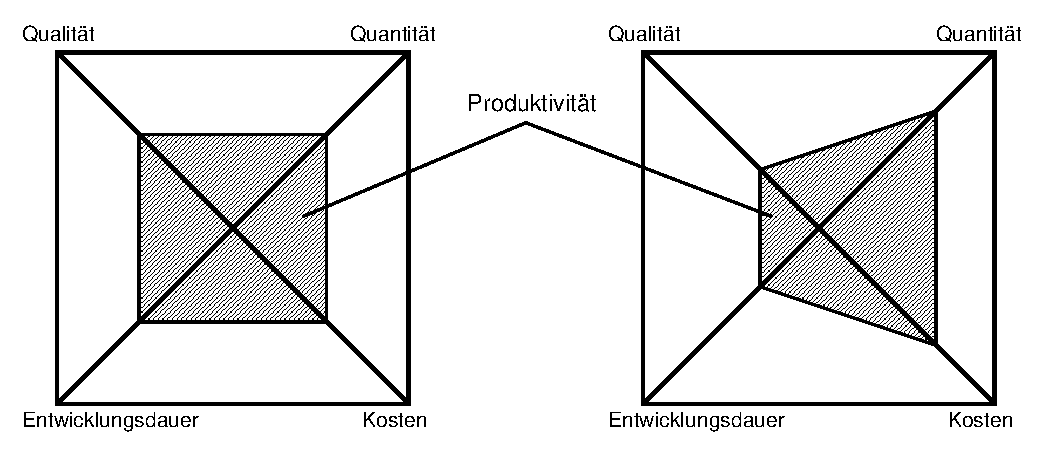
\includegraphics[width=0.8\textwidth]{Bilder/magicSquare} 
 \caption{Das magische Quadrat der konkurrierenden Ziele (als encapsulated
          postscript)  \label{magicSquare}}
\end{figure}
Auf Abbildungen kann nat�rlich auch referenziert werden \zb durch
"'\figref{magicSquare} auf Seite~\pageref{magicSquare}"'. Dies setzt allerdings
voraus, dass man ein Label definiert hat (\zb \verb+\label{magicSquare}+). Der Befehl
\verb+\figref{..}+ ist nicht von \LaTeX\ definiert sondern in der Datei {\code
Abkuerzugen.tex}.  Hier sieht man auch, wie man Anf�hrungszeichen schreibt \ldots
  
bla bla bla bla bla bla bla bla bla bla bla bla bla bla bla bla bla
bla bla bla bla bla bla bla bla bla bla bla bla bla bla bla bla bla
bla bla bla bla bla  

\newpage
\subsection{Noch ein paar Anmerkungen \label{Anmerkungen}} 

bla bla bla bla bla bla bla bla bla bla bla bla bla bla bla bla bla
bla bla bla bla bla bla bla bla bla bla bla bla bla bla bla bla bla

\begin{comment} 
\cbstart 
\ \vspace{0.5ex}
\hrule 
\ \vspace{0.5ex}

Dieser Abschnitt erscheint nur, wenn der Befehl \verb+\includecomment{comment}+ in
der \LaTeX -Hauptdatei steht.  Mit einem \verb+%+ -Zeichen kann er auskommentiert
werden. Dann verschwindet dieser Absatz aus dem Dokument.

Kommentar-Bereiche sind praktisch um Textteile im Dokument "'parken"' zu k�nnen. Bei
Bedarf kann man die Teile sichtbar bzw.\ unsichtbar schalten.  Der graue Balken am
Rand wird durch die Befehle \verb+\cbstart+ und \verb+\cbend+ erzeugt. Dazu muss das
Package \verb+changebar+ geladen werden. 
\ \vspace{0.5ex}
\hrule 
\ \vspace{0.5ex}\cbend
\end{comment} 

bla bla bla bla bla bla\footnote{Fu�noten sind ebenfalls problemlos m�glich.} bla bla
bla bla bla bla bla bla bla bla bla bla bla bla bla bla bla bla bla bla bla bla bla
bla bla bla bla bla bla bla bla bla bla bla bla bla bla bla bla bla bla bla bla bla
bla bla bla bla bla bla



 
\section{Stand der Technik \label{StandDerTechnik} }

\section{Methode \label{Methode} }

\section{Ergebnisse \label{Ergebnisse} }

\section{Zusammenfassung und Ausblick \label{ZusammenfassungUndAusblick} }


\begin{comment} 
\nocite{coulouris00, coulouris02} 
\end{comment} 

\addcontentsline{toc}{section}{Literatur} 
\bibliographystyle{alphadin} 
\bibliography{Literatur} 

\end{document} 


